\documentclass[14pt]{beamer}
\usepackage[T2A]{fontenc}
\usepackage[utf8]{inputenc}
\usepackage[english,russian]{babel}
\usepackage{amssymb,amsfonts,amsmath,mathtext}
\usepackage{cite,enumerate,float,indentfirst}
\usepackage{booktabs}

\graphicspath{{images/}}

\usetheme{Pittsburgh}
\usecolortheme{whale}

\setbeamercolor{footline}{fg=gray}
\setbeamertemplate{footline}{
  \leavevmode%
  \hbox{%
  \begin{beamercolorbox}[wd=.333333\paperwidth,ht=2.25ex,dp=1ex,center]{}%
    Куликов А.В., ABBYY-MIPT
  \end{beamercolorbox}%
  \begin{beamercolorbox}[wd=.333333\paperwidth,ht=2.25ex,dp=1ex,center]{}%
    Москва, 2017
  \end{beamercolorbox}%
  \begin{beamercolorbox}[wd=.333333\paperwidth,ht=2.25ex,dp=1ex,right]{}%
  Стр. \insertframenumber{} из \inserttotalframenumber \hspace*{2ex}
  \end{beamercolorbox}}%
  \vskip0pt%
}

\newcommand{\itemi}{\item[\checkmark]}

\title{\small{Японский: буквенные n-граммы для распознавания}}
\subtitle{\footnotesize{Контроль НИР}}
\author{\small{%
~Куликов А.В., гр. 397\\%
\emph{Руководитель:}~Андрианов А.И.}\\%
\vspace{30pt}%
ABBYY-MIPT%
\vspace{20pt}%
}
\date{\small{Москва, 2017}}

\begin{document}

\maketitle

\begin{frame}

\frametitle{Задача}
\begin{itemize}
    \item Japanese kanji/kana OCR.
    \item Существуют путающиеся символы, например:
    \begin{figure}[h]
        \center{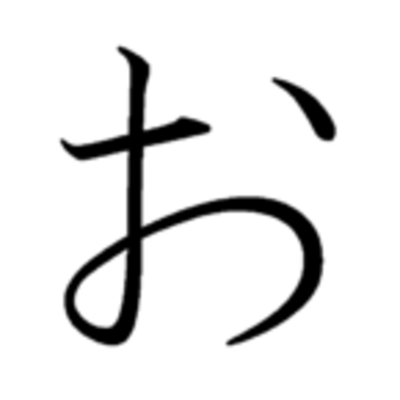
\includegraphics[scale=0.05]{KanaO}\ и 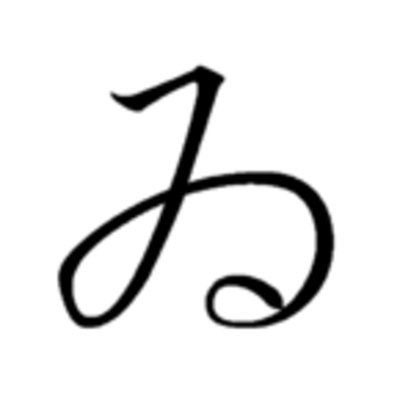
\includegraphics[scale=0.05]{KanaWi}}
    \end{figure}
    \item \emph{Цель работы: } построить и сравнить различные эвристики для исправления ошибок OCR, используя буквенную n-граммную модель японского языка.
\end{itemize}
\end{frame}

\begin{frame}
	\frametitle{Overview}
	\tableofcontents
\end{frame}

\section{Обработка корпуса, buckets}

\begin{frame}
\frametitle{Обработка корпуса}
Частоты символов в корпусе (всего 5.6E+8).

Размер алфавита $|\Sigma| = 7047$.

Это 33\% от Unicode CJK диапазона.
\begin{figure}[h]
	\center{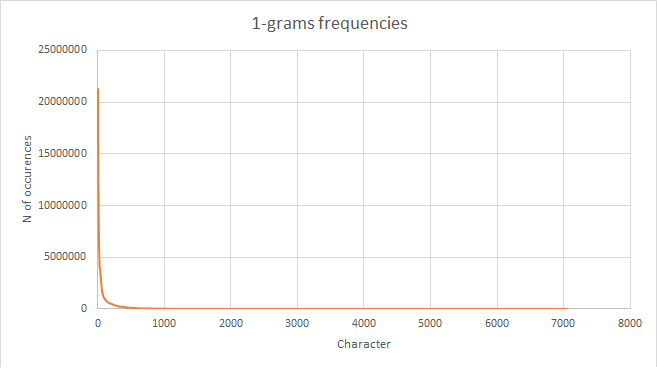
\includegraphics[scale=0.5]{1gramstatsbig}}
\end{figure}
\end{frame}

\begin{frame}
	\frametitle{1grams}
	Голова этого графика.
	\begin{figure}[h]
		\center{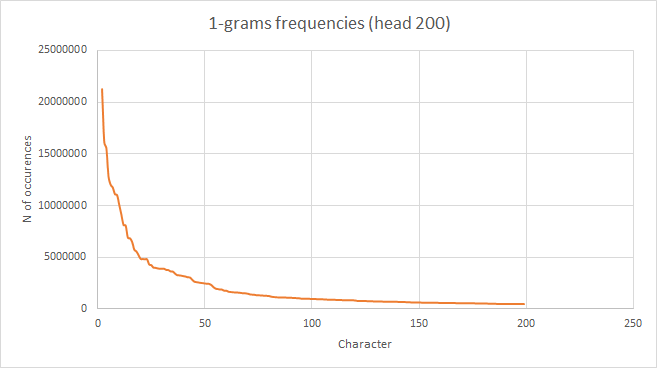
\includegraphics[scale=0.5]{1gramstatssmall}}
	\end{figure}
\end{frame}


\begin{frame}
	\frametitle{Buckets}
	Отбросим хвост с частотами $\leq 1000$ \\ ($<0,12\%$ корпуса, $|\Sigma^*| = 2600$).
	
	Заменим эти символы на 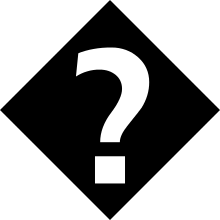
\includegraphics[scale=0.05]{fffd}.
	\begin{figure}[h]
		\center{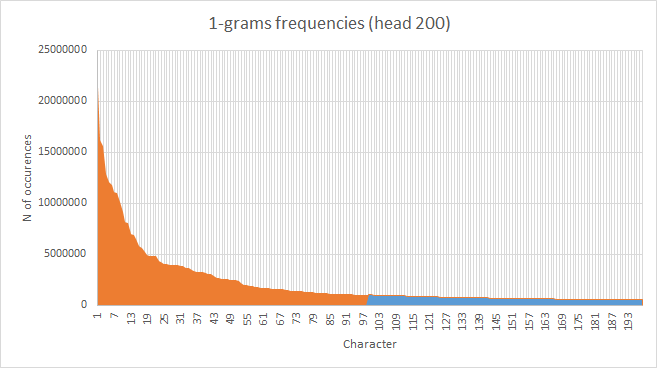
\includegraphics[scale=0.5]{1gramstatsbuckets}}
	\end{figure}

	Границу можно изменять.
\end{frame}

\section{Сбор статистики по n-граммам}

\begin{frame}
	\frametitle{Сбор статистики по n-граммам}
\begin{itemize}
	\item Храним статистику в боре (trie).
	\item Библиотека pygtrie даёт удобный функционал.
	\item $n_{max} = 7$.
	\item Размер бора 5GB.
	\item Учёт невстреченных символов: \\ Good-Turing, 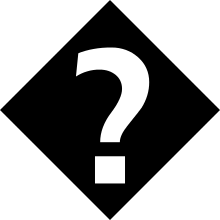
\includegraphics[scale=0.05]{fffd}.
\end{itemize}
\end{frame}

\begin{frame}
\frametitle{Trie stats}
\begin{center}
	\begin{tabular}{c|c}
		n	& Различных n-грамм \\ 
		1		&4430 \\
		2		&482607\\
		3		&3436987\\
		4		&10025503\\
		5		&19051342\\
		6		&28679559\\
		7		&37723274\\
	\end{tabular}
\end{center}
\end{frame}

\section{Шум как имитация ошибок OCR}


\begin{frame}
	\frametitle{Шум как имитация ошибок OCR}
	
	\begin{itemize}
		\item Ошибки OCR имитируются искусственным случайным зашумлением текста.
		\item Рандом зафиксирован.
		\item Новые списки путающихся символов:
		
		\begin{itemize} 	
			\item Ka-ga (диакритика) (KaGa);
			\begin{figure}[h]
				\center{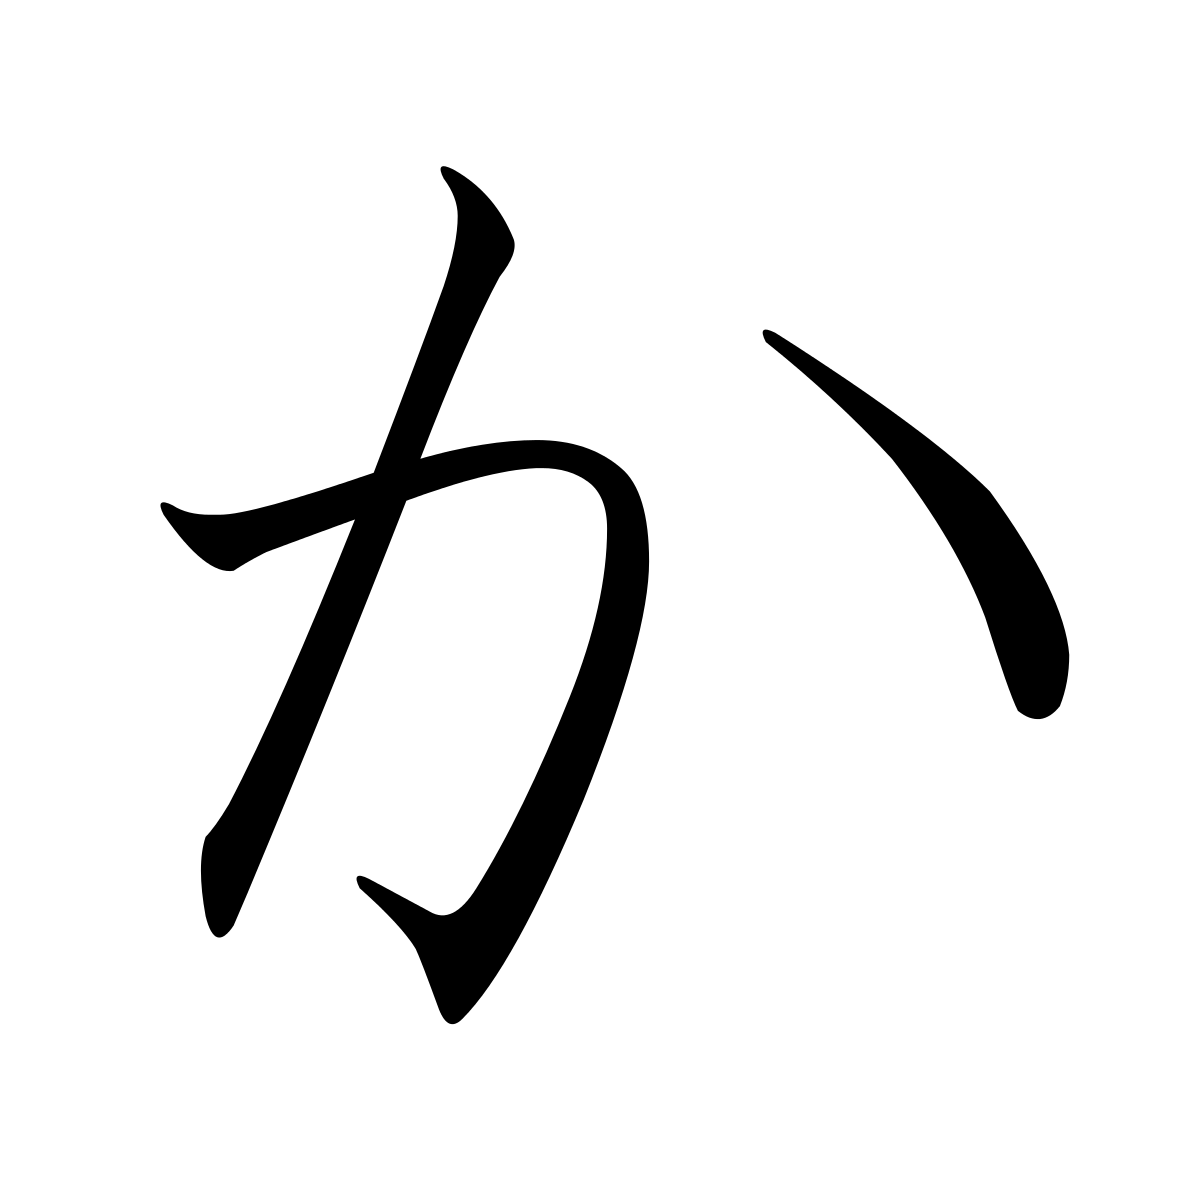
\includegraphics[width=30pt]{KanaKa}\ и 
\includegraphics[width=30pt]{KanaGa}}
			\end{figure}
			\item Halfwidth-fullwidth forms (HFW);
			\begin{figure}[h]
				\center{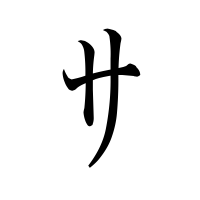
\includegraphics[width=30pt]{KanaA}\ и 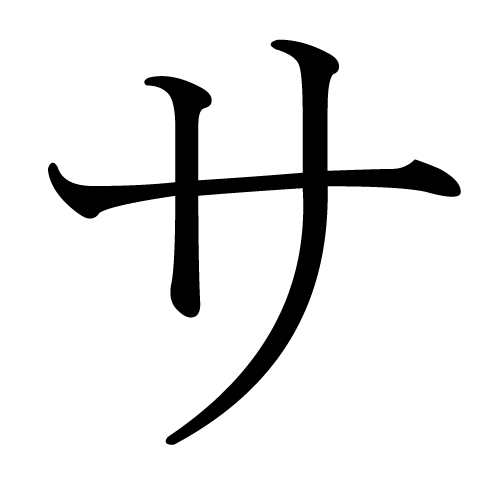
\includegraphics[width=30pt]{KanaAH}}
			\end{figure}
			\item Микс (Mix).
		\end{itemize}
	\end{itemize}
\end{frame}

\section{Модели оценки зашумлённого текста}

\begin{frame}
	\frametitle{Модели оценки}

\begin{itemize}
	\item 2-gram, 3-gram;
	\item Katz backoff (KBO) $n = 7$;
	\small
	\begin{equation*}
	P_{b0}\left( w_i | w_{i-n+1}...w_{i-1} \right) = 
	\end{equation*}
	\begin{equation*}
	\begin{cases}
	d_{w_{i-n+1}...w_i} \frac{C(w_{i-n+1}...w_i)}{C(w_{i-n+1}...w_{i-1})} &\text{if $C(w_{i-n+1}...w_i) > k$}\\
	\alpha_{w_{i-n+1}...w_{i-1}} P_{b0}\left( w_i | w_{i-n+2}...w_{i-1} \right) &\text{otherwise}
	\end{cases}
	\end{equation*}
	\item Stupid backoff (SBO) $n = 7$.
	$$ d_{w_{i-n+1}...w_i} = const $$
	$$ \alpha_{w_{i-n+1}...w_{i-1}} = const $$ 
\end{itemize}
\end{frame}

\section{Результаты работы моделей}

\begin{frame}
	\frametitle{Результаты работы моделей}
	Число -- процент угаданных предложений в тексте.

\begin{center}
	\begin{tabular}{c||c|c|c}
		Модель/Шум & KaGa 		& HFW 		& Mix \\
		\hrulefill & \hrulefill & \hrulefill& \hrulefill \\
		3-gram 	   &	82.3\%		&	85.6\%		&	83.7\%		\\
		Stupid BO  &	87.8\%		&	90.2\%		&	89.2\%		\\
		Katz BO    &	93.1\%		&	94.9\%		&		93.9\%	\\
		
	\end{tabular}
\end{center}	

В BO моделях есть возможность \\дальнейшей доводки параметров.
\end{frame}

\section{Эксперимент}

\begin{frame}
	\frametitle{Эксперимент с Zipf}
	
	\begin{figure}[h]
		\center{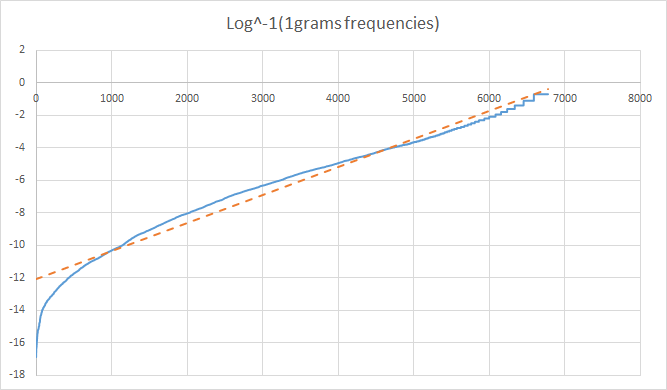
\includegraphics[scale=0.6]{Zipf}}
	\end{figure}
\end{frame}


\begin{frame}
	\frametitle{Эксперимент с Zipf}
	
	\begin{itemize}
		\item Как размер корпуса влияет на хвост распределения?
		
		\item Как мы можем имитировать большой корпус?
		
		\item Попробуем стохастически его уменьшать и посмотреть на графики.
	\end{itemize}
	
\end{frame}
\begin{frame}
	\frametitle{Планы на будущее}
	
	\begin{itemize}
		\item Тоньше настроить модель Katz BackOff.
		\item Попробовать имитировать больший корпус.
		\item Лучше визуализировать результаты.
		\item Писать текст.
	\end{itemize}
\end{frame}

\begin{frame}
\frametitle{Список литературы}
\footnotesize{
\begin{itemize}
  \item Foundations of Statistical Natural Language Processing / \\C. D. Manning, H. Schutze.
  \item Efficient In-memory Data Structures for N-Grams Indexing / \\D. Robenek, J. Platos, V. Snasel
\end{itemize}}
\end{frame}

\begin{frame}
\center{\huge
Спасибо
}
\end{frame}

\end{document} 